\documentclass[]{article}
\usepackage{lmodern}
\usepackage{amssymb,amsmath}
\usepackage{ifxetex,ifluatex}
\usepackage{fixltx2e} % provides \textsubscript
\ifnum 0\ifxetex 1\fi\ifluatex 1\fi=0 % if pdftex
  \usepackage[T1]{fontenc}
  \usepackage[utf8]{inputenc}
\else % if luatex or xelatex
  \ifxetex
    \usepackage{mathspec}
  \else
    \usepackage{fontspec}
  \fi
  \defaultfontfeatures{Ligatures=TeX,Scale=MatchLowercase}
\fi
% use upquote if available, for straight quotes in verbatim environments
\IfFileExists{upquote.sty}{\usepackage{upquote}}{}
% use microtype if available
\IfFileExists{microtype.sty}{%
\usepackage{microtype}
\UseMicrotypeSet[protrusion]{basicmath} % disable protrusion for tt fonts
}{}
\usepackage[margin=1in]{geometry}
\usepackage{hyperref}
\hypersetup{unicode=true,
            pdftitle={Understanding R\_0},
            pdfauthor={Chris H. Wilson, University of Florida},
            pdfborder={0 0 0},
            breaklinks=true}
\urlstyle{same}  % don't use monospace font for urls
\usepackage{graphicx,grffile}
\makeatletter
\def\maxwidth{\ifdim\Gin@nat@width>\linewidth\linewidth\else\Gin@nat@width\fi}
\def\maxheight{\ifdim\Gin@nat@height>\textheight\textheight\else\Gin@nat@height\fi}
\makeatother
% Scale images if necessary, so that they will not overflow the page
% margins by default, and it is still possible to overwrite the defaults
% using explicit options in \includegraphics[width, height, ...]{}
\setkeys{Gin}{width=\maxwidth,height=\maxheight,keepaspectratio}
\IfFileExists{parskip.sty}{%
\usepackage{parskip}
}{% else
\setlength{\parindent}{0pt}
\setlength{\parskip}{6pt plus 2pt minus 1pt}
}
\setlength{\emergencystretch}{3em}  % prevent overfull lines
\providecommand{\tightlist}{%
  \setlength{\itemsep}{0pt}\setlength{\parskip}{0pt}}
\setcounter{secnumdepth}{0}
% Redefines (sub)paragraphs to behave more like sections
\ifx\paragraph\undefined\else
\let\oldparagraph\paragraph
\renewcommand{\paragraph}[1]{\oldparagraph{#1}\mbox{}}
\fi
\ifx\subparagraph\undefined\else
\let\oldsubparagraph\subparagraph
\renewcommand{\subparagraph}[1]{\oldsubparagraph{#1}\mbox{}}
\fi

%%% Use protect on footnotes to avoid problems with footnotes in titles
\let\rmarkdownfootnote\footnote%
\def\footnote{\protect\rmarkdownfootnote}

%%% Change title format to be more compact
\usepackage{titling}

% Create subtitle command for use in maketitle
\providecommand{\subtitle}[1]{
  \posttitle{
    \begin{center}\large#1\end{center}
    }
}

\setlength{\droptitle}{-2em}

  \title{Understanding R\_0}
    \pretitle{\vspace{\droptitle}\centering\huge}
  \posttitle{\par}
    \author{Chris H. Wilson, University of Florida}
    \preauthor{\centering\large\emph}
  \postauthor{\par}
      \predate{\centering\large\emph}
  \postdate{\par}
    \date{March 20, 2020}


\begin{document}
\maketitle

\section{Introduction}\label{introduction}

If you are anything like me, you have been reading a \emph{lot} of
articles about the virology and epidemiology of SARS-COV2, the agent
behind the new disease Covid-19. Our knowledge about this virus is
developing rapidly - thankfully - however the scale of the public health
crisis we are facing is daunting. Rather than attempt any kind of
comprehensive analysis here, I want to help unpack one of the key pieces
of terminology that is being thrown around a lot, ``R naught'' (\(R_0\))
or the ``basic reproduction number''. This will be a mid-level
mathematical exposition, intended to make this epidemiological concept
intuitive to those with a decent generic quantitative fluency, but no
special training in disease ecology or related theory. It may even be
useful to those who have studied some population and disease ecology,
but are feeling rusty or never fully understood the logic behind the
models.

The basic ``toy model'' in epidemiology is the so-called ``SIR'' model,
standing for Susceptible/Infected/Recovered. This is the bread and
butter of modeling disease outbreaks in a population. In many cases, its
assumptions are way too restrictive to provide an accurate quantitative
predictive framework, but it is a useful framework to understand in
order to educate intuition. In the case of SARS-COV2, I am told that SIR
models actually do fit the data surprisingly well, at least within
cities, for reasons that will become clear. So the structure in this
little tutorial is simple: first we will derive SIR models from first
principles, and then second we will see where \(R_0\) comes from.

\section{Multiplicative Growth: From Discrete to
Continuous}\label{multiplicative-growth-from-discrete-to-continuous}

To begin, recall that the basic process underying biological growth is
multiplicative. That is to say, cells divide, organisms reproduce, and
so do viruses! This multiplication process tells us that, absent
structural constrains from outside, populations of cells, viruses and
organisms do not accumulate linearly over time but exponentially
(i.e.~non-linearly). In addition to multiplying, they spread.
Multiplicative growth is captured quite simply by the following
difference equation: \[\tag{1} X[t+1] = X[t] + \tau X[t]\] We can
rewrite this as: \[\tag{2} X[t+1] = (1 + \tau) X[t]\] and after
substitution \(\lambda = 1 + \tau\), we get:
\[\tag{3} X[t+1] = \lambda X[t]\] Here, \(\lambda\) represents the
multiplicative/geometric growth rate of the population \(X\) over some
discrete time interval indexed by \(t\). If we take \(\lambda = 2\), our
time-step is a doubling interval, and the population growth looks like

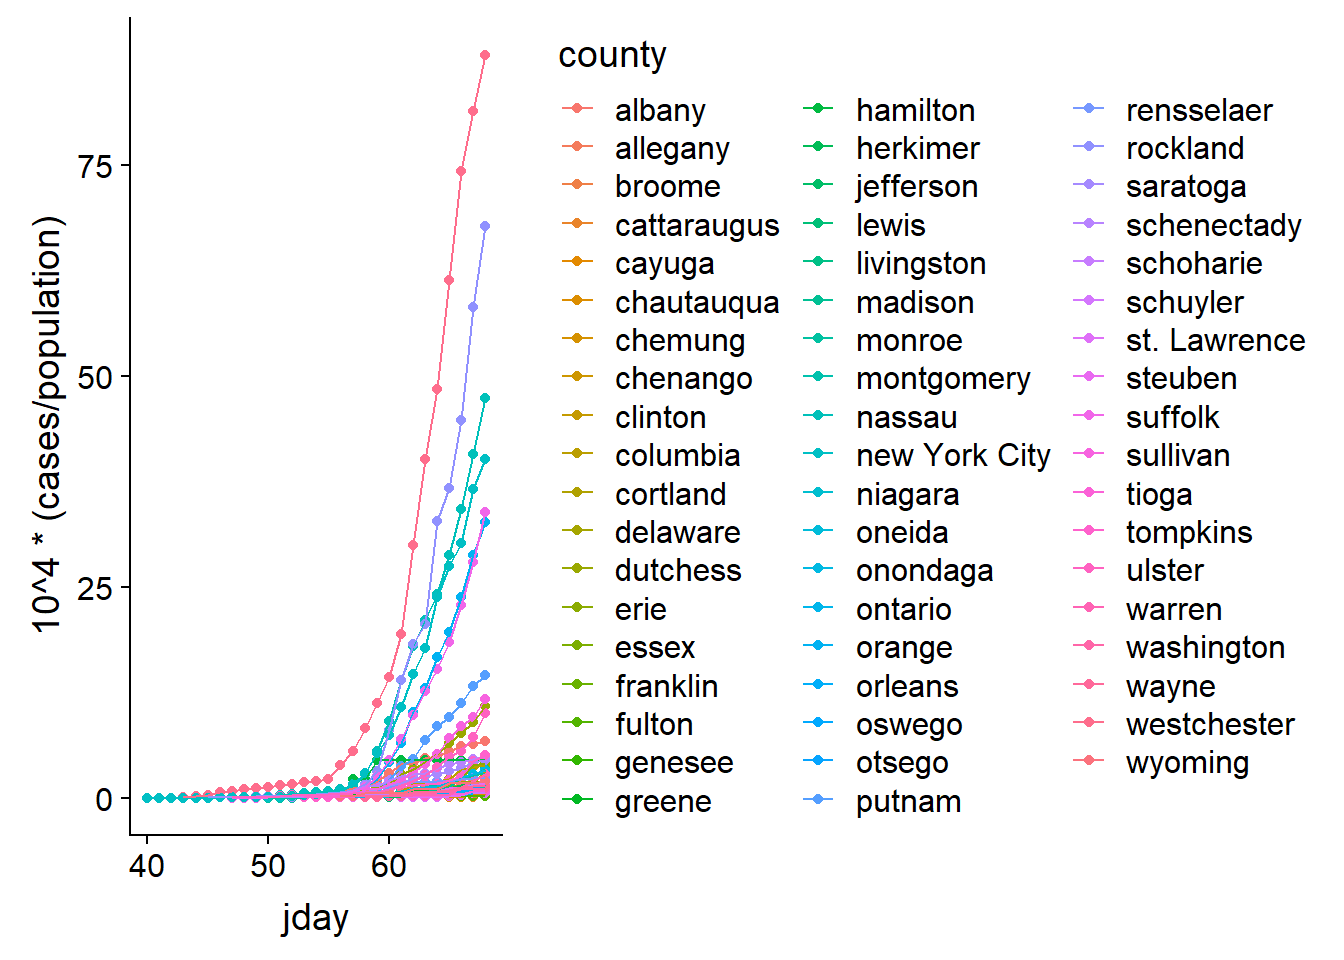
\includegraphics{R_0_files/figure-latex/unnamed-chunk-1-1.pdf}

Given \(T\) discrete time intervals, and an initial population \(X[0]\),
it is easily shown that our equation is
\[\tag{4} X[T] = \lambda^T X[0]\]

Now, discrete equations are nice, and in many ways most congenial for
biological processes. However, because we want to use the tools of
calculus and differential equations, we need to map this into continuous
form, which we do by defining an instantaneous growth rate \(k\), and
setting \(\lambda^T = e^{kT}\), hence \(k=log(\lambda)\), and our
continuous equation is: \[\tag{5} X[t] = e^{kt} X[0]\]. This turns out
to be the integral solution of the differential equation:
\[\tag{6} \frac{dX}{dt} = kX\] and with equation 6 we are finally ready
to jump into the SIR models, from which the concept of ``basic
reproductive rate'' is most easily derived.

\section{Deriving R\_0}\label{deriving-r_0}

Our first goal is to model how the number of infected people in a
population grows over time. To do this, we start with equation 6 and
then we make additional assumptions. The basic logic is this: you start
with an infected individual. That person then comes into contact with a
certain number of non-infected individuals at a certain rate. Call this,
``rate of contact'' (\(\kappa\)). In each contact, there is a certain
probability that the infection will be transmitted, ``transmission
probability''(\(\rho\)). When the number of infected individuals is
small relative to the total population (\(N\)), the growth in rate of
infections will be, to a high degree of approximation:
\[\tag{7} \frac{dI}{dt} = \kappa \rho I\]

As always with differential equations, it is helpful to be super clear
about the \textbf{dimensional analysis} (a hugely under-taught tool, see
Sanjoy Mahavan's excellent book ``Street Fighting Math''). On the left
hand side, we have something with dimensions of persons/time. On the
right hand side we have I (with dimensions `persons'), multiplied by
dimensionless probability \(\rho\), multiplied by a rate \(\kappa\). So
\(\kappa\) must ultimately have dimension of 1/time. Indeed, thinking it
through it is \#persons-contacted/(person-infected X time). The
dimensions of persons cancel, and we have 1/time, just as needed.

What equation 7 assumes so far is that \emph{every person contacted by
an infected individual is susceptible to infection}. However, as the
infected proportion of the population grows, this assumption breaks down
as the probability that an individual that is contacted is already
infected, or has recovered and is now resistant increases. We now
introduce a pool of susceptible individuals, ``S'', and we represent
this probability as \(S/N\) (a ratio that is also dimensionless). Since
this is dimensionless, we can simply stick it onto equation 7 no
problem, and we get:
\[\tag{8} \frac{dI}{dt} = \kappa \rho I \frac{S}{N}\]

Over time, \(\frac {S}{N}\) declines to 0, and the growth rate of
infections goes to zero. At this point, we need to point out that there
is a stringent assumption here. That is, this probability is homogeneous
across the population and can be represented by the proportion
\(\frac{S}{N}\). This is the so-called ``law of mass action'' imported
from equilibrial dynamics in chemistry and physics. In this context, it
requires the notion that populations are \emph{well mixed}. The real
world can get in the way of this being a good assumption when there is
strong spatial structure, strong heterogeneity in the population, and so
forth.

Another thing happens though. Infected individuals either die or recover
and become resistant. The simplest assumption here is that death and
recovery are also both first-order processes, so we subtract them from
the growth rate and complete our differential equation. For now, I am
going to pretend that no one dies (yay!) and people just become
resistant, as the math fundamentally does not change either way:
\[\tag{9} \frac {dI}{dt} = \kappa \rho I \frac{S}{N} - \nu I\]

Now, briefly, we must maintain the RHS with dimensions of persons/time,
so \(\nu\) is simply another rate with dimension of 1/time, and
represents rate of recovery into resistance.

And now we can see exactly what \(R_0\) is and where it comes from. An
individual does not stay infectious forever. They recover and become
resistant ``R'' instead, at the rate \(\nu\). But before they do this,
they are generating new infections at the rate \(\kappa \rho\). So if we
take the following ratio: \[\tag{10} \frac {\kappa \rho}{\nu}\], we have
a nice dimensionless number that represents the average number of new
infections per infected individual. This is \(R_0\) the ``basic
reproductive number''!

Return to the dimensionality for a second. It is customary to write
\(\kappa \rho\) as \(\beta\). Remember that this has a dimension of
1/time. Therefore, the ``typical time'' to a new infection is the
reciprocal or \(\frac{1}{\beta}\). Likewise, the ``typical time'' to
recovery is \(\frac{1}{\nu}\). ``\(R_0\)'' is clearly then the typical
time to recovery over the typical time to infection. A larger \(R_0\)
could arise from either recovery taking longer, time to infection being
shorter, or both.

Large \(R_0\) is bad. Small \(R_0\) is good.

In fact, we can now easily recover the single most important
epidemiological consequence of \(R_0\). Is the number of infected
individuals growing or declining? Our goal is to make a set of
interventions that turn equation 9 negative, thus guaranteeing the
decline of infected individuals, and eventual extinction of the
outbreak.

We re-write equation 9 using \(R_0\) from equation 10 and we get:
\[\tag {11} \frac {dI}{dt} = R_0 \nu I \frac{S}{N} - \nu I =  \nu I (R_0 \frac{S}{N} - 1) \]

At the beginning of an outbreak, where \(S \approx N\), this
differential equation is clearly positive when \(R_0\) \textgreater{} 1,
and negative when \(R_0\) \textless{} 1.

Here is the punchline: at the beginning of an outbreak, if you severely
limit average number of contacts between people, transmission
probabilities, or both, you can drive \(R_0\) below one and prevent the
outbreak from ever materializing. This is the goal of social distancing
measures. We can also be more surgical and effective at this if we
target infected individuals and their contacts for quarantine. This
requires widespread testing and is why the Trump administration's
response to Covid-19 is criminal malpractice.

As the pandemic proceeds, the number of susceptibles presumably
declines, which leads to self-limitation of the outbreak through the
ratio \(\frac{S}{N}\). This is the so-called ``herd immunity'' effect
that the British seem to be banking on. In better scenarios, we deploy
mass scale vaccination campaigns to drive enough people out of the ``S''
pool so that the equation goes negative that way. ``Herd immunity'' via
infection is a terribly risky proposition since it \textbf{requires} a
lot of people to get sick, and in the case of SARS-COV2 this is going to
mean lots of people dead both directly from the virus and indirectly
from a flooded healthcare system that can no longer take care of people
with all kinds of ailments. This, too, is criminal malpractice, given
all the uncertainties about Covid-19.

\section{Recovering the full SIR
model}\label{recovering-the-full-sir-model}

The rest of this tutorial will be brief. We complete our model with
understanding the disease by considering the three pools separately, in
the order S-I-R. \[\tag {12} \frac {dS}{dt} = - R_0 \nu I \frac{S}{N} \]
\[\tag {13} \frac {dI}{dt} = R_0 \nu I \frac{S}{N} - \nu I \]
\[\tag {14} \frac {dR}{dt} = \nu I \] This represents a system of three
coupled ODEs. We have removal of Susceptibles by infection, already
derived in detail. The initial condition is \(S[0] = N\). The dynamics
of the Susceptible pool have already been derived in detail. Then we
simply add an equation for the change in Recovered/Resistant pool which
receives everyone dropping out of the Infected pool.

And there you have it! This is the most basic foundation of infectious
disease epidemiology. Along the way, I hope the assumptions underlying
the epidemiology are more clear, as is the meaning of the ubiquitous
\(R_0\) term. In parting, I want to emphasize that \(R_0\) is NOT an
inherent property of a virus. It emerges dialectically from viral
biology interacting with human social behavior, which in turn is shaped
historically by culture, politics and economics.

We have a lot of leverage over epidemics. \textbf{Let us use our
collective agency to write a better history for this pandemic!}


\end{document}
